% !TEX program = xelatex
\documentclass[bachelor,openright,notchinese]{sustcthesis}
% 默认twoside 双面打印
% 将master修改为bachelor, doctor or master
% 要使用adobe字体,添加adobefonts选项
% 使用euler数学字体,如不愿使用,去掉euler
% 使用外文写作,请添加notchinese

% 设置图形文件的搜索路径
\graphicspath{{figures/}}

% 用到的宏包
\usepackage{algorithm2e}
% 阻止hyperref宏包影响tableofcontent内容
\makeatletter
\let\Hy@linktoc\Hy@linktoc@none
\makeatother

%%%%%%%%%%%%%%%%%%%%%%%%%%%%%%
%% 封面部分
%%%%%%%%%%%%%%%%%%%%%%%%%%%%%%
 % 中文封面内容
  \title{毕业论文}%一般情况下扉页和封皮、书脊共用一个标题文本,可以不用定义\spinetitle(仅硕博有用), \covertitle(本硕博均有用)和\encovertitle(仅本科有用)。特殊情况见下。
  %特殊情况1:本例中\title命令里含有换行控制字符,这会导致制作书脊的时候出现错误,例如如果你注释掉\spinetitle{...}这一行就会报错。这时需要定义一个不含换行等命令的\spinetitle,这并不表示\spinetitle里不能有任何命令——只能使用有限的命令。
  %特殊情况2:本例中标题过长,所以需要缩小书脊标题的字号。
  %特殊情况3:本例中中英文混排,由于tex竖排的原理限制,中英文基线不重合,所以需要人工调整英文的基线。具体调整量根据不同字体有所不同。
  %\covertitle{六次循环域}
  %\covertitle{中文题目第一行\\中文题目第二行}
  %不要在此调整封皮字体大小! Do not set Cover Page font size here!
  %特殊情况4:本例中\title中含有多个换行,导致标题超过了两行。根据制本厂规定,封皮标题不能超过两行。因此需要定义封皮使用的标题\covertitle. 如果你注释掉这一行,就会发现封皮不符合规定。
  %\encovertitle{On Cyclic Sextic Fields}
  %\encovertitle{English Title Line 1\\English Title Line 2\\English Title Line 3}
  %不要在此调整封皮字体大小! Do not set Cover Page font size here!
  %特殊情况5:仅本科生有用。本科封皮中有英文标题,不超过三行。与上类似。
  \author{张 \ 三 }
  \depart{计算机科学与工程}%系别,硕博请用系代号,本科请用全称如
  \major{计算机专业}%专业,硕博请用全称,本科不需要
  \advisor{XXXX \ 教授}
  % \coadvisor{XXX\ 教授,\ XXX\ 教授}%第二导师,没有请注释掉
  \studentid{XXXXX}%For bachelor only
  \submitdate{二〇一九年三月}

  % 英文封面内容
  \entitle{Bachelor Thesis}
  \enauthor{Junda Ai}
  \studentid{11711310}
  \endepart{Computer Science and Engineering}
  \enmajor{Computer Science and Technology}
  \enadvisor{Prof. Yepang Liu}
  % \encoadvisor{}
  % \encoadvisorsec{}
  \ensubmitdate{April, 2021}

\begin{document}

% 封面
\maketitle

%特别注意,以下述顺序为准,在对应部分添加文档部件,切勿颠倒顺序:
%本科论文的文档部件顺序是:
%    frontmatter:致谢、目录、中文摘要、英文摘要、
%    mainmatter: 正文章节
%    backmatter: 参考文献或资料注释、附录
%%%%%%%%%%%%%%%%%%%%%%%%%%%%%%
%% 前言部分
%%%%%%%%%%%%%%%%%%%%%%%%%%%%%%
\frontmatter
\makeatletter

\ifustc@bachelor
%%%%%%%%%%%%%%%%%
%本科论文修改这里
%%%%%%%%%%%%%%%%%
% 致谢
\chapter*{诚信承诺书}
\label{chap:honest}

\begin{enumerate}
\item 本人郑重承诺所呈交的毕业设计(论文),是在导师的指导下,独立进行研究工作所取得的成果,所有数据、图片资料均真实可靠。
\item 除文中已经注明引用的内容外,本论文不包含任何其他人或集体已经发表或撰写过的作品或成果。对本论文的研究作出重要贡献的个人和集体,均已在文中以明确的方式标明。
\item 本人承诺在毕业论文(设计)选题和研究内容过程中没有抄袭他人研究成果和伪造相关数据等行为。
\item 在毕业论文(设计)中对侵犯任何方面知识产权的行为,由本人承担相应的法律责任。
\end{enumerate}

\vskip 3\baselineskip


\begin{flushright}

作者签名: \underline{\hspace{4cm}}
\vskip \baselineskip
\underline{\hspace{1.4cm}}年\underline{\hspace{0.7cm}}月\underline{\hspace{0.7cm}}日

\end{flushright}

\chapter{Preface}
\label{chap:preface}
\vskip 28pt

This undergraduate graduation project is an extension of the previous work on Python API evolution conducted by Hengcheng Zhu and Zhaoxu Zhang of SUSTech class of 2020, which was summarized in their SANER 2020 paper \textit{How Do Python Framework APIs Evolve? An Exploratory Study}.

\begin{flushright}

Junda Ai

April, 2021 at SUSTech

\end{flushright}



%目录部分
%目录
\tableofcontents
%默认表格、插图、算法索引名称分别为“表格索引”、“插图索引”和“算法索引”
%如果需要自行修改lot,lof,loa的名称,请定义
%\ustclotname{...}
%\ustclofname{...}
%\ustcloaname{...}

% 表格索引
%\ustclot
% 插图索引
%\ustclof
%算法索引
%如果需要使用算法环境并列出算法索引,请加入补充宏包。
%\ustcloa

% 摘要
% \begin{cnabstract}
%     本文主要说明了....

% \keywords{关键词1, 关键词2}
% \end{cnabstract}

\begin{enabstract}

Python is a popular dynamic programming language that has thrived in the past decade with massive applications in various deciplines.

\enkeywords{Python, API Evolution, tree differencing, dynamic programming language}

\end{enabstract}
%此文件中含有中英文摘要

% \else
% 	%%%%%%%%%%%%%%%%%
% 	%硕博论文修改这里
% 	%%%%%%%%%%%%%%%%%
% 	% 摘要
% 	% \begin{cnabstract}
%     本文主要说明了....

% \keywords{关键词1, 关键词2}
% \end{cnabstract}

\begin{enabstract}

Python is a popular dynamic programming language that has thrived in the past decade with massive applications in various deciplines.

\enkeywords{Python, API Evolution, tree differencing, dynamic programming language}

\end{enabstract}
%此文件中含有中英文摘要
% 	% 目录
% 	\tableofcontents
% 	%默认表格、插图、算法索引名称分别为“表格索引”、“插图索引”和“算法索引”
% 	%如果需要自行修改lot,lof,loa的名称,请定义
% 	%\ustclotname{...}
% 	%\ustclofname{...}
% 	%\ustcloaname{...}

% 	% 表格索引
% 	\ustclot
% 	% 插图索引
% 	\ustclof
% 	%算法索引
% 	%如果需要使用算法环境并列出算法索引,请加入补充宏包。
% 	%\ustcloa

% 	%符号说明,需要加入补充包
% 	\begin{denotation}
\item[$\mathbb{Q}$] rational number field
\end{denotation}
%不是必需的,如果不想列出请注释掉
% \fi
\makeatother

%%%%%%%%%%%%%%%%%%%%%%%%%%%%%%
%% 正文部分
%%%%%%%%%%%%%%%%%%%%%%%%%%%%%%
\mainmatter
  \chapter{Introduction}
\label{chap:introduction}

Python is a popular dynamic programming language. Development frameworks written in Python thrived across multiple deciplines in recent decades, including \textit{TensorFlow} for deep learning, \textit{Pandas} for data analytics, and \textit{Django} for web services. The rule of Continuing Change discloses that programs either undergo continual change or become progressively less useful over time~\cite{evo-laws}. Akin to frameworks developed in other programming languages, Python frameworks obey this rule. However, the complication of framework release versions induce compatibility issues when the invoked APIs do not align with the APIs installed. Using the wrong version of framework APIs might induce compilation or runtime problems.

The goal of this project is to provide better API usage warnings for Python programs using static analysis prior to execution. Previously when client software developers called an obsolete API, Python runtime would print traces that report unavailable attribute in the module, which might be the consequence of multiple causes. We aims to understand the changes in framework implementations at a high level close to the framework developers' original intents, which requires us to understand compound changes in addition to atomic ones, and provide client programmers with useful suggestions such as "The API you used is renamed to ..." or "The API you used is obsoleted."
To summarize, this thesis accomplishes two major tasks:

\begin{itemize}
  \item Analyzed three real-world Python frameworks and collected common types of compound changes occurred in Python API evolution.
  \item Designed and implemented a tool to automatically detect compound changes classified in the above empirical study.
\end{itemize}

  \chapter{Background}
\label{chap:background}

\section{The Python Programming Language}
% A dynamic language; why calling missing API can only be reported until runtime

Python is dynamic programming language, the interpreter translates Python source code contained in a .py file to Python byte code and store it in a .pyc file. And it executes many common programming behaviors such as program extension, code insertion, object and definition extension, and type system modification which static programming languages perform during compilation~\cite{enwiki:dpl}. Depending on the arguments passed into a Python interpreter, it can read and execute single lines of command or command blocks interactively when connected to a tty device's standard input, or it can execute all statements\footnote{Here "statement" and "command" are used interchangeably} in a Python source file at once when called when the input is a file.

As a strongly typed programming language, data types of Python variables are tracked cannot be implicitly changed by the interpreter to compromise for the successful execution of the current command. But as a dynamically-typed programming language, programmers have great freedom of explicitly changing the type of a variable by assigning it new values, and variable types cannot be checked or retrieved until runtime. Due to lack of checkings during interpretation, errors such as invocations of undefined APIs, 

\section{Python API Evolution}
% Briefly summarize Hengcheng and Zhaoxu's findings

There are 14 types of change patterns found in Python framework evolution, 5 of which are specific to Python frameworks in comparison to Java frameworks due to the language features of Python. This evolution might induce crashes, including 10 types of runtime exceptions, or unexpected behaviors in client applications, more frequently than those in Java frameworks and Java client applications~\cite{DBLP:conf/wcre/ZhangZWTLX20}.

\subsection{Breaking and Non-breaking Changes}
% Distinguish between breaking/non-breaking changes

According to their effects, API changes can be classified into \textit{breaking changes} and \textit{non-breaking changes}~\cite{api-evo-refactoring}. Among the observed Python framework evolution patterns, some changes are not backward compatible and would induce compilation or runtime problems if the client program invokes obsolete APIs after updating dependent framework packages to newer versions. These changes that would lead to exceptions or unexpected behaviors are called breaking changes.

\subsection{Atomic and Compound Changes}
% Distinguish between atomic/compound changes

From the perspective of observing differences between two versions of a source file, atomic changes are insertion of new code and deletion of old code. This is different from the perspective of performing actions that produce those differences, in the case that an update action developer takes would be observed as a delete action and an insertion action in the aftermath, making it a compound change in our definition. An empirical study on compound changes by our definition will be discussed in chapter \hyperref[chap:compound-changes]{Compound Changes}.

Automation of detecting such compound changes is an important goal this project aims to achieve, as previous tools did not deliver. And comprehending the intents of such changes would help provide better API evolution and usage messages to client software developers which is the output of our tool.

\section{Tree Differencing}

The tree-to-tree correction problem was first studied in~\cite{tree-edit-p},~\cite{tree-correction-p}. It is a high-dimensional generalization of the string-to-string correction problem, and aims to determine the minimum cost of edit operations required to transform one tree to another. Since a Python source program could be parsed into an AST, tree-differencing algorithms could be applied to unmask the actual changes underneath different library\footnote{Here "library" and "framework" are also used interchangeably} release versions, hence providing client application developers with more thorough and accurate warnings and suggestions about which renewed API to use, rather than just printing generic warnings like missing module attributes.

In this project we use the tree-differencing algorithm described in~\cite{DBLP:conf/kbse/FalleriMBMM14}.

\subsection{Edit Action and Edit Script}

We take into account four types of edit actions: addition, removal, update, and move. For the AST of a program, the first two types of edit actions insert or delete tree nodes or subtrees to or from the AST. An update operation modifies the type of a tree node, resulting in a mutation of variable names, rvalue contents, arithmetic operators, comparison operators, conditional operators, and etc. Lastly, a move operation relocates a node or a subtree to another place in the AST. 

An edit script is a sequence of edit actions made to a source file that transform it between two versions.


  \chapter{Compound Change Patterns}
\label{chap:compound-changes}

To provide friendlier warning messages of API evolution, we need insight into what changes took place and the original intents of framework developers. This requires that we understand the compound changes which are observed as combinations of atomic changes between two versions of framework source code. Hence I studied real-world Python frameworks and summarized the types of compound changes observed in their evolution processes.

\section{Subject Selection}

I searched on the popular code hosting platform GitHub with the keywords \textit{rename}, \textit{relocation}, and \textit{relocate} under the topic topic:python. For every project hosted on GitHub, it provides three metrics to indicate the popularity of a project, namely stars, forks, and watches. We sorted the search results by a weighted measure of the three metrics, and selected the top repository from three popular categories: \textit{TensorFlow} in deep learning, \textit{Pandas} in data analytics, and \textit{Django} in web development. We analyzed the commit histories of those projects and collect a total of 535 commit records as the basis of our findings.

\section{Change Patterns}

\begin{enumerate}
  \item \textbf{Function Renaming}
  The most common function renaming would lead to missing module attribute error in old client code, and in the special case of adding or removing the leading underscore in a function's name, the function changes between public (no leading underscore in function name) and weakly private (with leading underscores in function name) \hyperref[fig:access-rename]{Figure 3.1}. We want to identify this kind of compound change in the hope of providing useful fix options to client programmers when they call an obsolete API, that we suggest using the matching API in the newer version of this framework, as we deduced that it is renamed. On the contrary, if the invoked API doesn't match any APIs in the renewed framework packages, we would inform the client developer that it is abandoned.

  \begin{figure}
    \caption{Change of leading underscores during function renaming}
    \label{fig:access-rename}
    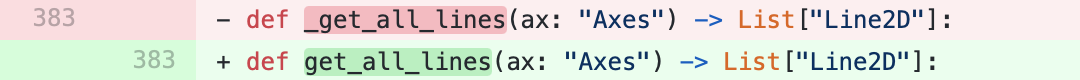
\includegraphics[width=\textwidth]{access-rename.png}
  \end{figure}

  \item \textbf{Parameter Compound Changes}
  Other than adding or deleting parameters of a function, which are atomic changes, the most common changes to parameters are to their data types and default values. These include modifying type hints in function definitions, and adding, deleting, or changing parameters' default values. Renaming parameters would not usually cause compatibility issues in client code, but there is also a special scenario of switching between \textit{self} and \textit{cls} in a class method definition. Placing \textit{self} as the first parameter of the function makes it an instance method, which could be invoked only after the class has been instantiated. While changing \textit{self} to \textit{cls} makes the function a class method, which can be called without an instance of the class.

  \item \textbf{Function Return Type Change}
  Changes of function return type are also based on type hints, including adding, deleting, and changing the function's return type hint.

  \item \textbf{Function Relocation}
  Relocating a function including migrating it to a different spot within the same source file and moving it to another source file. This adds workloads to our tool as cross-file relocation cannot be identified in the analysis of a single source file, which we rely on to detect the rest of the above compound changes.

\end{enumerate}

The above edit actions would usually be associated with other modifications to the functions' internal implementations. We need to take into consideration that changes in function implementations are the most common in framework evolutions, with or without changing the functions' names. We plan to match renamed APIs by generating and evaluating the edit script of two versions of a single source file.

  \chapter{Tool Design}
\label{chp:tool-design}

This is tool design.

\section{gumtree}

gumtree is an ast-differencing tool that can detect insert, delete, update, and move actions in python source files.

\section{Edit Script Evaluation}

I evaluate edit scripts generated by gumtree to decide whether a change is method renaming or not.

  \chapter{Tool Evaluation}
\label{chap:tool-evaluation}

In this section, I want to access the effectiveness of my tool on real-world data. I took advantage of the commit histories in the previous empirical study on Python framework evolution. For 50 commits of typical changes, including method renaming, parameter changes, parameter default value changes, and return annotation changes, among frameworks TensorFlow, Django, and Pandas, \textit{ccdetector} was able to correctly detect all the occurred changes and classify them in line with the intentions documented in the commit messages.

  \chapter{Conclusion}
\label{chap:conclusion}

In this thesis, we conducted an empirical study of commit histories of real-world Python frameworks to understand the high-level compound changes in Python framework API evolution. We collected 535 commits that represented typical compound change patterns in three popular Python libraries. Based on our empirical findings, we designed and implemented a tool that can automatically detect compatibility issues in client programs caused by compound breaking changes in dependent Python frameworks. \textit{And will evaluate it on real-world projects to measure its capability.}



%%%%%%%%%%%%%%%%%%%%%%%%%%%%%%
%% 附件部分
%%%%%%%%%%%%%%%%%%%%%%%%%%%%%%
\backmatter
  %结语

  % 参考文献
  % 使用 BibTeX
  % 选择参考文献的排版格式。注意ustcbib这个格式不保证完全符合要求,请自行决定是否使用
  \bibliographystyle{sustcbib}%{GBT7714-2005NLang-UTF8}
  \bibliography{bib/tex}
  \nocite{*} % for every item
  % 不使用 BibTeX
  % \include{chapter/bib}
  % 附录,没有请注释掉
  % \begin{appendix}

  % \include{chapter/appA}

  % \end{appendix}
  \begin{thanks}

  This work is supervised and guided by Professor Yepang Liu of Southern University of Science and Technology (SUSTech), Professor Ming Wen of Huazhong University of Science and Technology (HUST), Hengcheng Zhu of Hong the Hong Kong University of Science and Technology (HKUST), and Zhaoxu Zhang of the University of South California (USC). We discussed in group meetings on a weekly basis.

\vskip 18pt

\begin{flushright}

Junda Ai

May, 2021

\end{flushright}

\end{thanks}

\end{document}
